%\documentclass[a4paper,11pt]{memoir} 
\documentclass[oneside, a4paper,11pt]{memoir} 

\usepackage[utf8]{inputenc}
\usepackage[danish]{babel}
\usepackage[T1]{fontenc}
\usepackage[left=4.0cm, right=2.0cm, top=3.0cm, bottom=3.0cm]{geometry} 
\usepackage{amsmath,amssymb}																						

% SIUnitX  http://ctan.org/pkg/siunitx
\usepackage{siunitx,booktabs}		
\sisetup{per=slash}																						
\sisetup{per-mode = reciprocal}
\sisetup{inter-unit-product = \ensuremath{{}\cdot{}}}
\sisetup{output-decimal-marker = {,} }
\DeclareSIUnit{\kroner}{kr.}
\DeclareSIUnit{\LSb}{LSb}
\DeclareSIUnit{\cycles}{cycles}
\DeclareSIUnit{\div}{Div}

\usepackage{graphicx}
\newsubfloat{figure}% Allow subfloats in figure environment
\usepackage{dcolumn,booktabs}
\usepackage{url}
\usepackage{wrapfig}

% Redigere billed-/tabelteksterne.
\usepackage{caption}
\usepackage{subcaption}
\captionsetup{font=small,
labelfont={it,bf},textfont=sf,
format=hang}

% Packages for color handling
\usepackage[usenames,dvipsnames,svgnames,table]{xcolor}

\usepackage{threeparttable}

\usepackage{lscape}

\usepackage{enumitem}

% TODONotes http://ctan.org/pkg/todonotes
\usepackage{todonotes}
\usepackage{placeins}
\usepackage{lastpage}

\usepackage[hidelinks]{hyperref}  
\hypersetup{bookmarks=false}
\hypersetup{pdftitle={Embedded Modul\ae rt Audio Effekt System}} 
\hypersetup{pdfsubject={4. Semester Projekt, F18, Grp. [3]}}
\hypersetup{pdfauthor={J\"{o}rn Jacobi, Emil Schier Christiansen, Henrik Lund Hansen, Jes Rydall Larsen, Sonny Fink, Frederik Halling}}


% For includering af .pdf
\usepackage{pdfpages}

% Bibliografi
\usepackage{babelbib}
\bibliographystyle{abbrv}

% Noget forsideopsætning
\usepackage{soul} % lege lege
\sodef\an{}{0.2em}{.9em plus.6em}{1em plus.1em minus.1em}
\newcommand\stext[1]{\an{\scshape#1}}

% New commands 
\newcommand{\g}{9,82 \si{\meter\per\second\squared}}
\newcommand{\dcite}[1]{\quotedblbase{#1}\textquotedblright}
\newcommand{\husk}[2]{\todo[inline,color=green!40]{#1: #2}}
\newcommand{\jj}[1]{\todo[inline,color=green!40]{JJ: #1}}
\newcommand{\note}[1]{\todo[inline]{#1}}
\DeclareMathOperator{\lapl}{\mathcal{L}}

% Remove paragraph indentation for document
\setlength{\parindent}{0pt}
\newcommand\hcancel[2][black]{\setbox0=\hbox{$#2$}%
	\rlap{\raisebox{.45\ht0}{\textcolor{#1}{\rule{\wd0}{1pt}}}}#2} 

% Listings package
\usepackage{listings}

%Fede overskrifter
\usepackage{kpfonts}
\usepackage{calc}
\setSingleSpace{1.0}
\SingleSpacing
\definecolor{chaptercolor}{gray}{0.8}
% helper macros
%\newcommand\numlifter[1]{\raisebox{-2cm}[0pt][0pt]{\smash{#1}}}
\newcommand\numlifter[1]{\raisebox{-.8cm}[0pt][0pt]{\smash{#1}}}
\newcommand\numindent{\kern37pt}
\newlength\chaptertitleboxheight
\makechapterstyle{hansen}{
  \renewcommand\printchaptername{\raggedleft}
  \renewcommand\printchapternum{%
    \begingroup%
    \leavevmode%
    \chapnumfont%
    \strut%
    \numlifter{\thechapter}%
    \numindent%
\endgroup%
}
  \renewcommand*{\printchapternonum}{%
    \vphantom{\begingroup%
      \leavevmode%
      \chapnumfont%
      \numlifter{\vphantom{9}}%
      \numindent%
      \endgroup}
    \afterchapternum}
  \setlength\midchapskip{0pt}
  \setlength\beforechapskip{0.5\baselineskip}
  \setlength{\afterchapskip}{1\baselineskip}
  \renewcommand\chapnumfont{%
    %\fontsize{3cm}{0cm}%
    \fontsize{2cm}{0cm}
    \bfseries%
    \sffamily%
    \color{chaptercolor}%
  }
  \renewcommand\chaptitlefont{%
    \normalfont%
    %\huge%
    \LARGE%
    \bfseries%
    \raggedleft%
  }%
  \settototalheight\chaptertitleboxheight{%
    \parbox{\textwidth}{\chaptitlefont \strut bg\\bg\strut}}
  \renewcommand\printchaptertitle[1]{%
    \parbox[t][\chaptertitleboxheight][t]{\textwidth}{%
      %\microtypesetup{protrusion=false}% add this if you use microtype
      \chaptitlefont\strut ##1\strut}%
}}
\chapterstyle{hansen}
\aliaspagestyle{chapter}{empty} % just to save some space

%linje afstand
%\DisemulatePackage{setspace}
%\usepackage[nodisplayskipstretch]{setspace}
%\setstretch{0.5}
%\siglespacing
%\onehalfspacing                                       
%\doublespacing

%compile debug, check pdflatex time
\newcommand\showtimer{Timer: \the\numexpr\the\pdfelapsedtime*1000/65536 \relax}
%\pdfresettimer}
%\usepackage{fancyhdr}
%\pagestyle{fancy}
%\fancyfoot[CE,CO]{\showtimer}




\begin{document}
% --------- Frontpage ------------------
\begin{titlingpage}
\thispagestyle{empty}
\centering
{ \setlength{\baselineskip}{24pt}
{\Huge \stext{Embedded Modul\ae rt Audio Effekt System} \par
%\textit{\&}\par
%\stext{Analogier}
}\par
\stext{Indlejrede systemer og signalbehandling - F18}
\vspace*{1cm}



\par

\includegraphics[width=0.5\linewidth]{./billeder/SDU_segl1.png}
\par\vspace*{2\onelineskip}
\stext{4. Semester Projekt}\par

\large\stext{J\"{o}rn Jacobi -- 230674}\par
\large\stext{Emil Schier Christiansen -- ddmmyy}\par
\large\stext{Henrik Lund Hansen -- 270494}\par
\large\stext{Jes Rydall Larsen -- 140893}\par
\large\stext{Sonny Fink -- ddmmyy}\par
\large\stext{Frederik Halling -- ddmmyy}\par

\vfill
\vspace*{2\onelineskip}
\stext{Gruppe 3}\par
\stext{Vejleder: Ib Refer }\par
\stext{1. februar - 25. maj 2018}\hfill
%\stext{24. maj 2013}\hfill
\par\vspace*{2\onelineskip}
\small
\stext{M\ae rsk Mc-Kinney M\o ller Instituttet}\par
\stext{Syddansk Universitet}
\enlargethispage{2\onelineskip}
}
\end{titlingpage}


% --------- Abstract -------------------
\newpage
\thispagestyle{empty}
\renewcommand{\abstractnamefont}{\normalfont\bfseries}
\renewcommand{\abstracttextfont}{\normalfont}
\begin{abstract}
Resumé	
\end{abstract} 

% --------- Thanks ---------------------
%\newpage\thispagestyle{empty}\null\vfill\begin{center}\emph{Thanks note goes here}\end{center}

%---------- Underskrift
%\newpage\thispagestyle{empty}\null
\section*{Underskrifter}
\vspace{3ex} \hfill Underskrevet d. 24/05-2018\\

\newlength{\streg} \setlength{\streg}{0.49\linewidth}
\vspace*{\fill} \rule{\streg}{1pt} \hfill \rule{\streg}{1pt}\\
\begin{minipage}[b]{\streg}
 \centering
 \rule{0pt}{4ex}
 J\"{o}rn Jacobi \\
 {\footnotesize (230674) (jojac11@student.sdu.dk)}
\end{minipage}
\hfill
\begin{minipage}[b]{\streg}
 \centering
 Emil Schier Christiansen \\
 {\footnotesize (ddmmyy) (xxx@student.sdu.dk)}
\end{minipage}

\vspace*{\fill} \rule{\streg}{1pt} \hfill \rule{\streg}{1pt}\\
\begin{minipage}[b]{\streg}
 \centering
 \rule{0pt}{4ex}
 Henrik Lund Hansen \\
 {\footnotesize (ddmmyy) (xxx@student.sdu.dk)}
\end{minipage}
\hfill
\begin{minipage}[b]{\streg}
 \centering
 Jes Rydall Larsen \\
 {\footnotesize (ddmmyy) (xxx@student.sdu.dk)}
\end{minipage}

\vspace*{\fill} \rule{\streg}{1pt} \hfill \rule{\streg}{1pt}\\
\begin{minipage}[b]{\streg}
	\centering
	\rule{0pt}{4ex}
	Sonny Fink \\
	{\footnotesize (ddmmyy) (xxx@student.sdu.dk)}
\end{minipage}
\hfill
\begin{minipage}[b]{\streg}
	\centering
	Frederik Halling  \\
	{\footnotesize (ddmmyy) (xxx@student.sdu.dk)}
\end{minipage}\newpage\thispagestyle{empty}\null\vfill

%---------- Forord
\newpage
\thispagestyle{empty}
\chapter*{Forord}\label{chap:forord}
\addcontentsline{toc}{chapter}{Forord}
Dette projekt er udarbejdet af seks ingeniør-studerende på 4. semester for Elektronik og Datateknik på Syddansk Universitet. 
Projektet er udført i perioden d. 1. februar til d. 25. maj 2018. 
Projektet er udført under vejledning af Ib Refer. Gruppen takker for støtten gennem forløbet. 

\husk{NOTE}{I nogle rapporter ønsker forfatterne at indsætte et forord. Dette kan være i form af en tak til
	samarbejdspartnere, en dedikation af projektet til bestemte personer, eller fordi de ønsker at
	redegøre for ændrede forhold i forbindelse med rapporten.
	Et forord er ikke en obligatorisk del af et projekt. Det er som navnet siger ”før ordet”, dvs. før selve
	rapporten og kan ofte udelades.}

\subsection{Læsevejledning}
Rapporten bør læses fra start til slut som et samlet og sammenhængende værk. 
Som udgangspunkt antages det, at læseren har et fagligt kompetenceniveau som en studerende på 4. semester med linjefag indenfor elektronik og datateknik.

\subsection{Typografiske konventioner}
Her er en kort oversigt over de typografiske konventioner der anvendes i denne rapport.

\bigskip

\begin{tabular}{l p{0.6\linewidth}}
	\textit{Kursiv tekst}			& Angiver filnavne i den tilhørende kodebase samt fremhævelse af ord eller fagudtryk. \\
	\textbf{Fed tekst}				& Bruges til a fremhæve produkt eller system specifikke betegnelser.\\
	\texttt{Konstant brede tekst}	& Anvendes til kildekode eksempler. Ligeledes anvendes afgrænsende områder.\\
	\emph{Fremhævet tekst}		    & Bliver brugt når der gives en kort introduktion til hvert kapitel.\\
\end{tabular}

\subsection{Typografi}
Rapporten er fremstillet i \LaTeX - Memoir, sat i 11 pt. Computer Modern.\\
Antal sider : \pageref{LastPage}

% Removed for single page
%\newpage\thispagestyle{empty}\null\vfill

%---------- Indholdsfortegnelse  ---
\newpage
\tableofcontents*		

% Removed for single page										
%\newpage

%\DoubleSpacing	
%---------- Kalibrerings side --------
%\input{config/kalib}
%\newpage

%---------- Indledning -------------
\chapter{Indledning}
\vspace*{0.5 cm}
\emph{Kapitel intro}

\section{Formål}
\begin{itemize}
	\item Et projekt er semester krav som man går til eksamen.
	\item Hvor faglighederne indgår.
\end{itemize}

Formålet med projektet er at undersøge hvordan lyd kan behandles og manipuleres ved at bruge digital signalbehandling i et embedded miljø.
Hvordan samples signaler korrekt.
Løsningen skal opbygges som en modulær løsning, således at nye "lydmoduler" kan efter udvikles.
Styringen af modulerne skal kunne forgå igennem EMP boardet - her tænkes det at kunne anvende HID styringen dette board stiller til rådighed og som sammen LCDen skal udgøre en platform til UI'en. 


\section{Problemformulering}


\begin{itemize}
	\item Realtids lydbehandling 
	\item Digital filter design
	\item Analog filter design
	\item OS krav / design
	\item Test krav og eftervisning af forventede
\end{itemize}

\section{Projektafgrænsning}
\begin{itemize}
	\item Produktet er ikke udviklet som et slutprodukt.
\end{itemize}

\section{Kravspecifikation} 
\begin{itemize}
	\item Der skal anvendes vores ARM Cortex-M4 TI launchpad 
	\item Sampling Fs = 44,1 kHz Stereo (CD standard)
	\item FreeRTOS anvendes som OS	 
\end{itemize}

\section{Løsningsmodel}

\section{Proces- og arbejdsmetode}
							

\listoftodos
%\input{config/howto} 

%---------- Chapter ----------------
%\input{section/kap_equalizer}

%---------- Parts ----------------
%\input{section/equalizer}

\chapter{Anti aliasing filtre}\label{kap:aafiltre}
\vspace*{.5cm}

\section{Modtager af indgangssignal}
\husk{JES}{Hvad hedder denne del egentligt?}
Systemet skal kunne modtage et signal fra en lydkilde, som afspiller lyd i det menneskeligt hørbare område. 
Før signalet kan videreføres til anti aliasing filtrene, skal der være en mulighed for eventuelt at forstærke signalet med en operationsforstærker. 
På den måde kan en fuld opløsning opnås ved den senere AD konvertering. 
\newline
Et almindeligt analogt lydsignal har generelt frekvenser mellem 20Hz og 20kHz, som svarer til det menneskeligt hørbare område. 
Signalets spænding varierer for forskellige kilder. 
Der findes ingen officiel standard, men en del forbruger-elektronik har typisk en maksimal amplitude på 0,447V.\cite{wikiLine} 
\newline
Til forstærkningen benyttes en aktiv operationsforstærker med 3,3V single-supply. 
Men indgangssignalet fra lydkilden vil svinge omkring 0V. 
Derfor skal signalet have et offset, da signalet ellers vil blive klippet hver gang det går under 0V, da operationsforstærkeren ved single-supply ikke har mulighed for at have negative udgangssignaler. 
Det ønskes at indgangssignalet har mulighed for at svinge både så højt og lavt som muligt, så offsettet designes til at være symmetrisk, med respekt til  forsyningsspændingen. 
\begin{equation}
	{V_{offset}} = \frac{V_{supply}}{2} = \frac{3,3\text{V}}{2} = 1,65\text{V}
\end{equation}
Ved et offset på 1,65V kan signalet ideelt have en maksimal amplitude på 1,65V. 
%Herfra skal den valgte operationsforstærkers output swing i forhold til dens forsyningsspænding trækkes fra. (vender tilbage til det her når op-amp skal vælges)
Ved at opbygge en spændingsdeler, kan offsettet skabes. Kredsløbet ses på figur \ref{fig:modtagerKreds}.

\subsubsection{Valg af operationsforstærker til forstærkning af indgangssignalet}
Operationsforstærkeren som skal forstærke signalet vælges ud fra en række krav. 

\begin{itemize}
	\item Forstærkeren skal kunne forsynes med  single-supply 3,3V
	\item Båndbredden skal være minimum 44,1 kHz.
	\item Rail to rail voltage swing skal være så stort som muligt. 
	\item Slew rate skal være hurtig nok til at signalet ikke forvrænges. 
	\item Komponenten skal være tilgængelig som SMD komponent. 
\end{itemize}
Den nødvendige slew rate kan beregnes ved formel \ref{eq:slewrate}.\cite{slewrate}
\begin{equation}
\label{eq:slewrate}
\text{Slew rate} = 2 \pi \cdot f_{maks} \cdot V_{maks} = 2\pi \cdot 44,1\text{kHz} \cdot 1,65\text{V} = 0,46\text{V/\micro S}
\end{equation}
\husk{JES}{Er det egentligt kun 20kHz her?}
Ud fra kravene vælges operationsforstærkeren AD8031 som SMD komponent. 
Forstærkeren kan operere ved en single-supply forsyning ned til 2,7V, har 80MHz -3dB båndbredde ved en forstærkning på 1 og en slew rate på 30V/\micro S. 
Forstærkerens output swing ligger inden for 20mV af rail-spændingen. Ved 3,3V ligger spændingsvidden således fra 0,02V til 3,28V. 
Forstærkerens specifikationer overgår kravene med en stor margen. 
Det var ikke muligt at finde en anden operationsforstærker som var tilgængelig som SMD, der både havde en acceptabel slew rate, samt muligheden for en single-supply forsyningsspænding på 3,3V. 
Havde der været mere tid, kunne det have været bestilt hjem. 
\husk{JES}{Der er muligvis én der lever op til krav... Tjekker op på det. }

\subsubsection{Beregning af forstærkning}
For at forstærke signalet, opsættes operationsforstærkeren som en ikke-inverterende forstærker. 
Da indgangssignalets maksimale amplitude vil variere alt efter input, skal forstærkningens styrke kunne justeres. 
Derfor sættes en variabel modstand i serie med feedback-modstanden. 
Det ses på figur \ref{fig:modtagerKreds}. 
Den variable modstand kan gå fra at være tæt på kortsluttet og op til 100k$\Omega$.
For at undgå en kortslutning fra operationsforstærkerens output og til den inverterende indgang, er den variable modstand sat i serie med en feedback-modstand på 5k$\Omega$. 
$R_2$ er valgt til 47k$\Omega$, så modstanden matcher modstanden fra højpasfilteret. \husk{Jes}{Vender tilbage til de 47k.}
I formel \ref{eq:Aminfors} og \ref{eq:Aminfors} ses den mulige maksimum- og minimumsforstærkning.

\begin{equation}
\label{eq:Aminfors}
A_{maks.} = 1 + \frac{R_{feedback} + R_{variabel}}{R_2} = 1 + \frac{5\text{k} \Omega + 100\text{k} \Omega}{47\text{k} \Omega} = 3,23
\end{equation}
\begin{equation}
\label{Amaksfors}
A_{min.} = 1 + \frac{R_{feedback}}{R_2} = 1 + \frac{5\text{k} \Omega}{47\text{k} \Omega} = 1,11
\end{equation}

\subsubsection{Højpas filter-design}
Mellem inputtet og operationsforstærkeren sidder en kapacitor, som blokerer for al DC fra indgangssignalet. 
Som det ses på figur \ref{fig:modtagerKreds}, vil kapacitoren og modstandene fra offsettet udgøre et højpas filter. 
Filterets knækfrekvens sættes så lavt, at alle frekvenser i det hørbare område ikke påvirkes. 
Ved AC-analyse kortsluttet forsyningen. Derfor sidder modstandene $R1$ og $R2$ parallelt.
Det endelige kredsløb er kopieret, således der er to udgange for at opnå stereo. 
\begin{equation}
f_c = \frac{1}{2\pi R C} = \frac{1}{2 \pi \frac{1}{\frac{1}{47k \Omega}+\frac{1}{47k \Omega}}  470\text{nF}} = 14,1\text{Hz}
\end{equation}

\begin{figure}[h]
\caption{Kredsløbet for modtageren af indgangssignalet.}
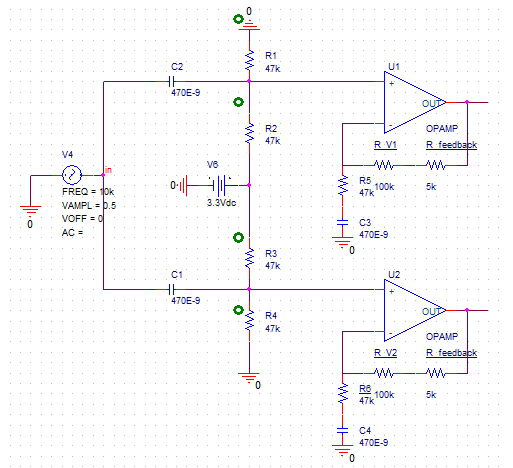
\includegraphics[width=0.8\linewidth]{./billeder/Modtager.png}
\label{fig:modtagerKreds}
\end{figure}

\husk{Jes}{Hvis der er problemer med antal sider, kan der henvises til et bilag med det samlede print i stedet.}

\section{Anti aliasing filtre}

\section{Filter print design}

\chapter{Reverb effektmodul}\label{chap:reverb}
Reverb, rumklang, er resultatet af lydbølger som bliver reflekteret tilbage af samtlige overflader med forskellige vinkler.\newline
Rumklang er resultatet af lydbølger som bliver reflekteret af samtlige overflader i et rum, derved bygges der en masse reflektioner op hvis amplitude falder mod $0$ som de bliver absorberet af overfladerne i rummet.\newline
Der er to primære metoder for implementeringen af en digital reverb effekt.
Der er convolution (foldnings) reverben og den algoritmiske reverb.
\subsection{Convolution reverb}
Reverberation, rumklang, er en tidsinvariant effekt, hvilket betyder at det ikke har nogen betydning, hvornår en tone bliver spillet, det vil ultimativt resultere i præcis den samme reverberation. \newline
Med tidsinvariante systemer kan de karakteriseres ved deres impulsrespons.
Convolution reverbs virker ved at lave en foldning af rummets impulsrespons og det lydsignal der sættes på indgange n til reverben.\newline
Dette skaber en realistisk rumklangseffekt, fordi impulsen i dette tilfælde vil være en lyd som holder samme energiniveau ved alle frekvenser.
Efter impulsen bliver spillet vil den blive reflekteret rundt i rummet.
Nogle af reflektionerne møder mikrofonen med det samme mens andre bliver ført rundt i rummet og amplituden af signalerne går mod $0$ pga. overfladerne af objekterne i rummet absorbere energien fra dem.\newline
Multiplikering af hver punkt af impulsresponset med amplituden af samplet giver så rummets respons til den sample.
Dette gøres for hver sample af inputtet og giver overlappende responser som så adderes og resulterer i rumklang.
En ulempe ved convolution reverbs er, at der skal mange beregninger til for at få resultatet.
Hvert sample skal individuelt multipliceres med hvert sample af impulsresponset og adderes.
Hvis der haves $N$ samples og impulsresponset er $M$ samples lang skal der udføres $N+M$ multiplikationer og additioner.
F.eks. hvis der haves et impulsrespons på 1 sekund og der samples med $44.1\si{kHz}$, skal der udføres næsten 2 milliarder multiplikationer og additioner i sekundet.
Antallet af multiplikationer og additioner kan dog reduceres drastisk ved at arbejde i frekvensdomænet i stedet for, da foldning i frekvensdomænet er multiplikation.

Fordelen ved convolution reverbs er at ethvert rum i verden kan imiteres, hvis impulsresponset for det valgte rum haves.\newline
Derudover kan man opfinde rum ved at syntetisere et impulsrespons.

\subsection{Algoritmisk reverb}
En algoritmisk reverb virker ved at bruge flere forskellige delays og feedback loops til at opbygge en serie af ekkoer, som dør ud over tid.
Det er sammensætningen af de basale byggeblokke som giver karakteristikken på rummet der emuleres.\newline
Et eksempel på en simpel algoritmist reverb effekt er all-pass filteret.
%insert billede af all-pass filter
Her bliver samplet feeded forward til outputtet så lyden bliver spillet med det samme.
Derudover smides samplet ind i en delay buffer.
Rumklangen skabes så af samples fra delay bufferen, som fungerer som opbygningen af ekkoer og feedback loopet som agerer som absorptionen for at skabe aftagende ekkoer.





\section{Implementering af reverb}
%Der blev valgt en algoritmisk reverb, da det blev vurderet at den var 
\subsection{Kode}
\lstset{frame=tb,
	language=c,
	aboveskip=3mm,
	belowskip=3mm,
	showstringspaces=false,
	columns=flexible,
	basicstyle={\small\ttfamily},
	numbers=none,
	numberstyle=\tiny\color{gray},
	keywordstyle=\color{blue},
	commentstyle=\color{dkgreen},
	stringstyle=\color{mauve},
	breaklines=true,
	breakatwhitespace=true,
	tabsize=3,
	texcl=true
}
\begin{lstlisting}
void mod_reverb_effekt( fp_sample_t *in, fp_sample_t *out)
{
	if(is_sw1_pressed)
	{
		const float in_gain = -0.25;
		const float fb_gain = -0.05;
		const uint16_t delay = 2000;

	fp_sample_t fp_sample;
	sample_buffer_get(&fp_sample);

	fp_sample.left_fp32 = ((in->left_fp32 * in_gain) + ((in->left_fp32 + fp_sample.left_fp32) * fb_gain));
	fp_sample.right_fp32 = ((in->right_fp32 * in_gain) + ((in->left_fp32 + fp_sample.right_fp32) * fb_gain));

	sample_buffer_put_z(&fp_sample, delay);

	out->left_fp32 = in->left_fp32;
	out->right_fp32 = in->right_fp32;
	}
	else
	{
	out->left_fp32 = in->left_fp32;
	out->right_fp32 = in->right_fp32;
	}
}
\end{lstlisting}

%Koden er implementeringen af allpass filteret.\newline
Koden er implementeringen af et all-pass filter.
Først hentes en sample ind fra sample bufferen.
Input samplet bliver ganget med feedback gainet og input gainet og lægges DELAY pladser frem i sample bufferen.\newline
Der opbygges en masse ekkoer, da funktionen bliver kaldt hver gang der kommer et sample ind.\newline
Disse ekkoer der ligger på i sample bufferen bliver lagt sammen med 
%Efter hvert SAMPLE_BUFFER_PUT_OUT kald inkrementeres HEAD pointeren i bufferen, således

%Input samplet sættes så på output, således at 
%Det virker ved at funktionen tager et input sample, og tilfører de specificerede gains til det.
%Dernæst skriver den det resulterende sample ud i en samplebuffer på den plads, der svarer til det specificerede delay.
%Reverbet forekommer så som 

%---------- Chapter ----------------
\chapter{Diskussion og vurdering}\label{kap:diskussion}
\vspace*{.5cm}


%MCU


%DSP
En betydeligt mere realistisk rumklangs/ekko effekt kunne have været opnået med et ''convolution reverb``, dette ville dog have krævet en bedre microcontroller med højere clock og mere plads til at gemme data og der blev derfor i stedet valgt at anvende algoritmiske løsninger.

%En af de begrænsende faktorer ved implementering af effektmodulerne er den korte tid, der er til at foretage beregninger mellem samples bliver taget til de skal ud igen.
%Den begrensede tid kan skabe et problem for store beregninger der kan tage lang tid, hvis en sådan beregning på signalet ikke bliver færdiggjort før samplet skal ud igen bliver signalbehandlingen ikke korrekt udført, eller det kan resultere i et delay af signalet, hvilket ikke ønskes. \husk{Emil}{jeg her helt bestemt ikke tilfreds med denne sætning...}
%Af hensyn til dette er det vigtigt at lave beregninger så hurgtigt og effiktivt som muligt.

%En betydelig begrænsning i implementering af effektmodulerne er den korte tid mellem at en samples modtages og sendes ud igen.
%Dette betyder at  meget store og eller komplicerede beregninger simpelthen ikke kan udføres hurtigt nok til at undgå forsinkelser der kan opfattes af det menneskelige øre.
%Det er derfor vigtigt at optimere og begrænse alle beregninger så de bruger den mindste tid muligt. 
%\husk{Sonny}{Har skrevet en alternativ udgave af teksten herover}
%Ved både Echo- og Reverbeffektmodulerne er dette tilfældet, da der ved hvert sample kun skal laves et ganske lille antal simple beregninger.
%I Echoeffektmodulet er bliver et sample blot ganget med en gain/decay \note{hvad kalder vi det?} og derefter adderet til en værdig i en buffer.
%Reverbeffekten opnås ved en lignende metode, det er næmlig valgt at benytte en algoritmisk reverb frem for convolution reverb, altså ved foldning.
%Dette er valgt, selvom der i teorien ville kunne opnås en bedre, mere realistisk, reverbeffekt ved convolution reverb.
%Valget er truffet, da det ville betyde at der skulle foretages flere beregninger imellem input og output samples.
%Hvilket ville betyde, at der ville være en risiko for ikke at nå beregningerne, uden en stor mængde planlægning af beregningerne.
%Denne metode har også behov for en større mængde hukommelse end den algoritmiske reverb effekt.
%Dette er også en af grundende til, at dette valg blev truffet. 
%Da det endte med en pladsmangel på microcontrolleren, når der skal ligge flere forskellige moduler på.

	
						
%---------- Chapter ----------------
\chapter{Konklusion} \label{kap:konklusion}

							
\husk{Jes}{'test' skal naturligvis flyttes til bilag. Men der vil dokumentet ikke compilere? Mangler 'begin document' eller noget... }
\section{Test af det samlede system}
\label{kap:test}
Testens formål er at udføre en vector network analyse af det samlede system for at finde systemets amplitude-karakteristik. 
Det samlede system består af modtageren af indgangssignalet, anti-aliasing filtrene for den ene kanal, Tiva-kittet med EMP board og microcontroller, DAC, rekonstruktionsfilteret for den ene kanal og udgangskredsløbet. 

\subsection{Udstyr}
\begin{itemize}
	\item Bode 100 med tilhørende udstyr
	\item Èn computer med Bode Analyzer Suite installeret
	\item To oscilloskop-prober
	\item Skillekondensator
\end{itemize}

\subsection{Fremgangsmåde og forsøgsopstilling}
Opsæt Bode 100 uden noget tilsluttet. 
Åben Bode Analyzer Suite, og vælg en Gain/Phase-analyse under Vector Network Analysis. 
Analysen sættes op med følgende indstillinger:
\begin{multicols}{2}
\begin{itemize}
	\item Startfrekvens: 10 Hz
	\item Slutfrekvens: 50 kHz
	\item Minimum 401 data points
	\item Source level: 0 dBm
	\item Attenuator på receiver 1 \& 2: 10 dB
	\item Receiver bandwidth: 100 Hz
	\item External reference på CH1 \& CH2
\end{itemize}
\end{multicols}
Vælg Trace 1 til Magnitude (dB). \newline
Med Bode Analyzer suite laves en kalibrering af Bode 100, når udgangen og indgangene på Bode 100 er koblet sammen. 
Skillekondensatoren skal være på udgangen. \newline
Opsæt det samlede system som vist på figur \ref{fig:lol}. 
Bode 100's udgang med skillekondensator og CH1 kobles til indgangen på den ene kanal af det samlede system. 
CH2 kobles til udgangen af det samlede system for den tilsvarende kanal. 
Analysen kan nu udføres. 

\subsection{Resultat af test}
Datasættet for resultatet af testen kan ses i den vedhæftede fil \textit{'habibi.csv'}. 
\husk{Jes}{Filnavn skal rettes her!}
\begin{figure}[h]
	\caption{Overføringsfunktionen af det samlede system.}
	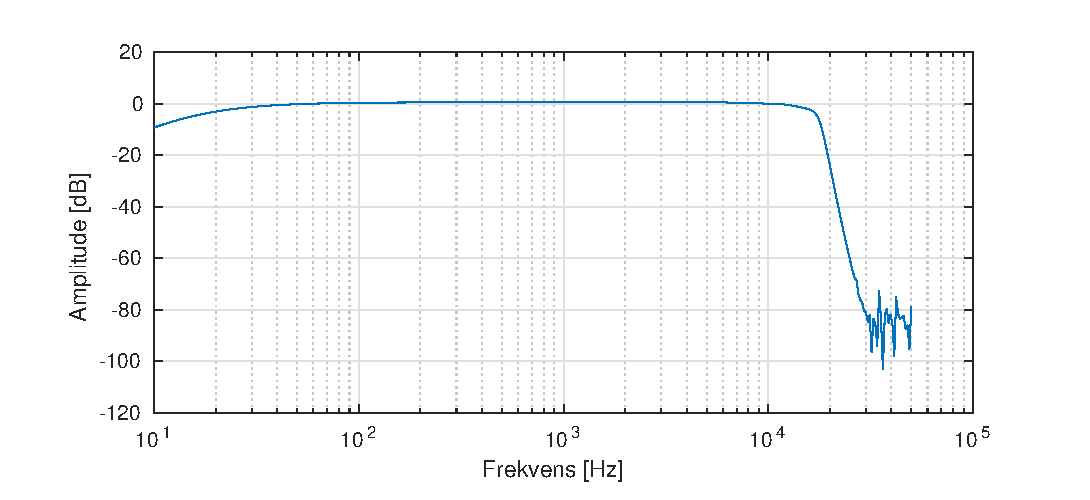
\includegraphics[width=1\linewidth]{./billeder/tf_samletsystem.eps}
	\label{fig:tf_samletsystem}
\end{figure}

\section{Test af anti-aliasing filtre}
%Formål her.
Testen følger samme fremgangsmåde, som ved testen af det samlede system. 
Dog testes udelukkende anti-aliasing filtrene.  

\SingleSpacing

\nocite{*}
\bibliography{rapport}\label{bilag:litteratur}
%\listoffigures
%\listoftables

%--------- Bilag -------------------
\appendix
\chapter{Bilag}
%\chapter{Ordliste} \label{bilag:ordliste}

\begin{table}[h!]
	\caption{Ordliste}
	\label{tab:ordliste}
	\begin{threeparttable}
		\begin{tabular}{l p{0.7\textwidth}}
			\toprule
			\textbf{Ord}      & \textbf{Beskrivelse}   \\ 
			\midrule
			AA			& Antialiasing.\\
			ADC			& Analog digital converter (Eng.)\\
			ANSI		& American National Standards Institute (Eng.)\\
			API			& Grænseflade på en computer der tillader én softwarekomponent at kommunikere med en anden\tnote{a}\\
%			CLI			& Commandline interface (Eng.)\\
			DAC			& Digital analog converter (Eng.)\\
%			Latency		& (Eng.) Tidsforsinkelsen imellem stimulans og respons.\\ 
			LCD			& Liquid crystal display (Eng.) \\
			MCU       	& Micro Controller Unit (Eng.). Microcontroller eller mikroprocessor. \\
%			Periferienhed & Selvkørende hardwaremodul i mikrocontrollerens arkitektur.\\
			Preemptive	& (Eng.) Afbrydelse af task fra fx. en scheduler.\\
			PWM			& Pulse Width Modulation (Eng.) \\
			SAR			& Successive Approximation Register (Eng.)\\
%			Shell		& Brugerinterface (CLI) til operativsystemets funktionalitet.\\
			SPI			& Serial Peripheral Interface (Eng.)  \\
			UART		& Universal asynchronous receiver and transmitter (Eng.)\\
			\bottomrule
		\end{tabular}
	
		\begin{tablenotes}
			\item[a] \textit{Den Danske Ordbog - \url{http://ordnet.dk/}}
		\end{tablenotes}
	\end{threeparttable}
\end{table}

%\input{section/symbol}
%\chapter{Pin mapping} \label{bilag:pinmap}
\begin{table}[h!]
	\centering
	\caption{Pin konfiguration af Tiva LaunchPad, EMP print og Projekt print}
	\label{tab:pin_mapping}
	\begin{threeparttable}
		\begin{tabular}{l l l l l l}
			\toprule
			\textbf{Tiva Pin\tnote{a}} 	& 
			\textbf{GPIO\tnote{b}}  	&
			\textbf{Tiva\tnote{c}} 		& 
			\textbf{EMP\tnote{d}}  		&
			\textbf{Projekt\tnote{e}} 	\\ 
			\midrule
			1.01 &      & 3V3  	& +3.3VDC		& 3V3		\\
			1.02 &  PB5 &      	& PB5			& (SPI2) FSS/$\overline{CS}$		\\
			1.03 &	PB0 &	   	& PB0			& Debug P0	\\
			1.04 &	PB1 &      	& PB1			& Debug	P1	\\
			1.05 &	PE4 &	   	& Audio Out     & Audio In Left	\\
			1.06 &	PE5 &	   	& Audio In		& Audio In Right \\
			1.07 &	PB4 &	   	& PB4			& (SPI2) CLK/SCK		\\
			1.08 &	PA5 &	   	& DIGI A		& 					\\
			1.09 &	PA6 &	   	& DIGI B    	& 								\\
			1.10 &	PA7 &	   	& DIGI P2		& 								\\
			\midrule
			2.01 &     	& GND  	& GND  			& GND 						\\
			2.02 & PB2 	&      	& T3CCP0 (PWM)	& 							\\
			2.03 & PE0 	&	  	& KEYB G 		&								\\
			2.04 & PF0 	& SW2	& 				&								\\
			2.05 &     	& RESET	& 				&								\\
			2.06 & PB7	&		& PB7			& (SPI2) TX/SDI					\\
			2.07 & PB6	&		& PB6			& (SPI2) RX (NA)				\\
			2.08 & PA4 	&      	& KEYB F 		&						\\
			2.09 & PA3 	&		& KEYB E    	& 						\\
			2.10 & PA2  &		& KEYB D		& 						\\
			\midrule
			3.01 &		& 5V0	& +5VDC			&	+5VDC							\\
			3.02 &		& GND	& GND			&	GND							\\
			3.03 & PD0	&(R10)	&				&								\\
			3.04 & PD1	&(R9)	&				&								\\
			3.05 & PD2	&		& LCD RS		& 				\\
			3.06 & PD3	&		& LCD E			& 						\\
			3.07 & PE1	&		& KEYB H		& 							\\
			3.08 & PE2	&		& KEYB J		&							\\
			3.09 & PE3	&		& KEYB K		&								\\
			3.10 & PF1	&LED (R)& LED R			&								\\
			\bottomrule
		\end{tabular}
	
		\begin{tablenotes}
			\item[] Forsættes på næste side...
		\end{tablenotes}
	\end{threeparttable}
\end{table}
\newpage
\begin{table}[ht]
	\centering
	\caption{Pin konfiguration af Tiva LaunchPad, EMP print og Projekt print}
	\begin{threeparttable}
		\begin{tabular}{l l l l l l}
			\toprule
			\textbf{Tiva Pin\tnote{a}} 	& 
			\textbf{GPIO\tnote{b}}  	&
			\textbf{Tiva\tnote{c}} 		& 
			\textbf{EMP\tnote{d}}  		&
			\textbf{Projekt\tnote{e}} 	\\ 
			\midrule
			4.01 & PF2	&LED (B)& LED Y			&								\\
			4.02 & PF3	&LED (G)& LED G			&								\\
			4.03 & PB3	&		& PB3			&	$\overline{LDAC}$							\\
			4.04 & PC4	&		& LCD D4		& 			\\
			4.05 & PC5	&		& LCD D5		& 				\\
			4.06 & PC6	&		& LCD D6		& 				\\
			4.07 & PC7	&		& LCD D7		& 				\\
			4.08 & PD6	&		& Status LED	& 		\\
			4.09 & PD7	&		& 				&								\\
			4.10 & PF4	& SW1	& 				&								\\
			\bottomrule
		\end{tabular}
		
		\begin{tablenotes}
			\item[x] Jumper på EMP printet skal sættes til. \textbf{J5 pin 1-2} og \textbf{J4} skal fjernes.
			\item[a,b] JP1-4 på Tiva LaunchPad \cite[Afsnit 2.1.5 s. 9]{spmu296}.
			\item[c] On-board funktion \cite[Afsnit 2.1.5 s. 9]{spmu296}.
			\item[d] EMP print funktionalitet er beskrevet i tilhørende diagram \cite{emp-diagram}.
			\item[e] Projekt , se bilag \ref{bilag:diagram}.
		\end{tablenotes}
	\end{threeparttable}
\end{table}
%\input{section/cd_indhold}
%\chapter{Stykliste} \label{bilag:styklister}
\begin{table}[h!]
\small
%\centering
\caption{Stykliste for diagrammet \ref{bilag:diagram}.}
\label{tab:styklister}
\begin{threeparttable}
\begin{tabular}{p{0.22\linewidth}p{0.1\linewidth}p{0.18\linewidth}p{0.05\linewidth}p{0.1\linewidth}p{0.1\linewidth}p{0.05\linewidth}}
%\begin{tabular}{ l l l l l l l }
\toprule
\multicolumn{1}{l}{\textbf{Komponent}}       &
\multicolumn{1}{l}{\textbf{Værdi}}       &
\multicolumn{1}{l}{\textbf{Type}}       &
\multicolumn{1}{l}{\textbf{Tol.}} &
\multicolumn{1}{l}{\textbf{Klasse}} &
\multicolumn{1}{l}{\textbf{Bemærkning}} &
\multicolumn{1}{l}{\textbf{Type / Lev.}}  \\ 
\hline
R1, R2, R4, R6, R7,& $\SI{47}{\kilo\ohm}$ & Keramisk SMD & $\pm 1\%$ & $\SI{0.25}{\watt}$ & 100ppm/\si{\celsius} & (c) \\
R9 &&&&&& \\
R3, R8 & $\SI{5}{\kilo\ohm}$ & Keramisk SMD	& $\pm 1\%$ & $\SI{0.25}{\watt}$ & 100ppm/\si{\celsius}  & (c) \\
R5, R10 & $\SI{100}{\kilo\ohm}$ & Potentiometer	& $\pm 1\%$ & $\SI{0.25}{\watt}$ & 100ppm/\si{\celsius}  & (c) \\
R11X*4, R12X*4, & $\SI{10}{\kilo\ohm}$ & Keramisk SMD	& $\pm 1\%$ & $\SI{0.25}{\watt}$ & 100ppm/\si{\celsius}  & (c) \\
R21X*4, R22X*4, &&&&&& \\
R31X*4, R32X*4 &&&&&& \\
\midrule
C1, C2, C4, C5 & $\SI{490}{\nano\farad}$ & Keramisk SMD & $\pm 5\%$ & 100 \si{\volt} &  & (c)\\
C3, C6, C15X*4, & $\SI{0,1}{\micro\farad}$ & Keramisk SMD & $\pm 5\%$ & 100 \si{\volt} &  & (c)\\
C25X*4, C35X*4 &&&&&&\\
C7, C8 & $\SI{1}{\micro\farad}$ & Keramisk SMD & $\pm 5\%$ & 100 \si{\volt} &  & (c)\\
C2U1 & $\SI{10}{\micro\farad}$ & Keramisk SMD & $\pm 5\%$ & 100 \si{\volt} &  & (c)\\
C2U2 & $\SI{100}{\nano\farad}$ & Keramisk SMD & $\pm 5\%$ & 100 \si{\volt} &  & (c)\\
C11X*4, C33X*4 & $\SI{220}{\pico\farad}$ & Keramisk SMD & $\pm 5\%$ & 100 \si{\volt} &  & (c)\\
C12X*4, C37X & $\SI{100}{\pico\farad}$ & Keramisk SMD & $\pm 5\%$ & 100 \si{\volt} &  & (c)\\
C13X*4 & $\SI{470}{\nano\farad}$ & Keramisk SMD & $\pm 5\%$ & 100 \si{\volt} &  & (c)\\
C14X*4, C17X*4, & $\SI{2,2}{\nano\farad}$ & Keramisk SMD & $\pm 5\%$ & 100 \si{\volt} &  & (c)\\
C18X*4, C22X*4 &&&&&& \\
C16X*4, C28X*4 & $\SI{470}{\pico\farad}$ & Keramisk SMD & $\pm 5\%$ & 100 \si{\volt} &  & (c)\\
C21X*4, C23X*4, & $\SI{47}{\nano\farad}$ & Keramisk SMD & $\pm 5\%$ & 100 \si{\volt} &  & (c)\\
C32X*4 &&&&&& \\
C24X*4, C34X*4, & $\SI{1}{\nano\farad}$ & Keramisk SMD & $\pm 5\%$ & 100 \si{\volt} &  & (c)\\
C36X*4 &&&&&&\\
C26X*4, C27X*4, & $\SI{15}{\pico\farad}$ & Keramisk SMD & $\pm 5\%$ & 100 \si{\volt} &  & (c)\\
C38X*4, C39X*4 &&&&&&\\
C29X*4 & $\SI{4,7}{\nano\farad}$ & Keramisk SMD & $\pm 5\%$ & 100 \si{\volt} &  & (c)\\
C31X*4 & $\SI{10}{\nano\farad}$ & Keramisk SMD & $\pm 5\%$ & 100 \si{\volt} &  & (c)\\
\midrule
IC5*4, IC6*4, IC7*4, IC11, IC12 & AD8031 & OP Amp &  &  &  & (a) \\
U1 & MCP4922-E/P & DAC &  &  &  & (d) \\
SV1, SV2 & TM4C123GH6PM & &  &  &  & (b) \\
X\textunderscore IN & KLBR4 & & & & Surface mount & (e) \\
X\textunderscore OUT & KLBR4 & & & & Surface mount & (e) \\
\hline
\bottomrule
\end{tabular}
\begin{tablenotes}
%\textbf{Typ/Lev.}
\item[a] (), (Analog Devices)
\item[b] (), (Texas Instruments, http://www.ti.com/lit/ds/symlink/tm4c123gh6pm.pdf)
\item[c] (), (Phillips)
\item[d] (), (Microchip)
\item[e] (), (Lumberg)
\item[u] Ukendt
\end{tablenotes}
\end{threeparttable}
\end{table} 

%\input{section/tidsplan}
%\input{section/diagrammer}
%\chapter{Diagram} \label{bilag:diagram} % Denne side skal ikke bruges, den skal blot fjernes og erstattes med digrammet


\end{document}
